\Chapter{A TikZ és eszközkészlete}

% Kb. 8 oldal

\Section{Ábrák szerkesztése LaTeX-ben}

A rajzolás megkönnyítése érdekében a TikZ-t használjuk, amely egy frontend réteg a PGF-hez. Egy ábrát létrehozni azt jelenti, hogy egyenes vagy görbe vonalak sorozatát rajzoljuk meg. A TikZ parancsaira és szintaxisára olyan források voltak hatással, mint a METAFONT, a PSTricks és még sokan mások.

\noindent
A pontok és koordináták megadására a TikZ egy speciális szintaxist biztosít. A legegyszerűbb, ha kerek zárójelben vesszővel elválasztott két dimenziót használunk, például (4pt, 6pt). Ha az egység nincs megadva, akkor az xy-koordináta rendszerének alapértelmezett értékeit használjuk. Ez azt jelenti, hogy az egységnyi x-vektor 1 cm-rel jobbra, az egységnyi y-vektor pedig 1 cm-rel felfelé halad. 

\Section{A TikZ elemei}

\SubSection{Használata}
% usepackage, telepítés, útmutatók

Először is be kell állítanunk a környezetünket. Kezdetnek a következőképpen állítjuk be a fájlunkat:

\begin{lstlisting}[style=latex]
\documentclass{article}
\usepackage{tikz}
\begin{document}
	<content>
\end{document}
\end{lstlisting}

\noindent
Ezután kezdjük el az ábrák létrehozását. 


\SubSection{Szintaxis}
% Alapvető nyelvi elemek bemutatása

A szabály az, hogy minden TikZ grafikus rajzoló parancsnak a \lstinline{\tikz} parancs argumentumaként vagy a {tikzpicture} környezeten belül kell előfordulnia. 

\noindent
A {tikzpicture} környezet \LaTeX\ változata a következő:

\begin{lstlisting}[style=latex]
\begin{tikzpicture}[options]
	<content>
\end{tikzpicture}
\end{lstlisting}


\noindent
A környezeten belül megadott összes opció a teljes képre vonatkozik.

\noindent
A TikZ-ben minden ábra alapvető építőeleme a vonal. Egy vonalat a kezdőpont koordinátáinak megadásával kezdünk, mint például (0,0), majd hozzáadunk egy vonal bővítő műveletet, a legegyszerűbb csak "--". A műveletet ezután a következő koordináta követi. Minden útvonalnak pontosvesszővel kell végződnie. Az vonal megrajzolásához a \lstinline{\draw} parancsot használjuk.

\noindent
Például a (0,0), (0,1), (1,0) pontok közötti háromszög megrajzolásához azt írhatjuk, hogy:

\begin{lstlisting}[style=latex]
\tikz\draw (0,0) -- (0,1) -- (1,0) -- (0,0);
\end{lstlisting}
vagy

\begin{lstlisting}[style=latex]
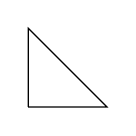
\begin{tikzpicture}
	\draw (0,0) -- (0,1) -- (1,0) -- (0,0);
\end{tikzpicture}
\end{lstlisting}


\begin{tikzcode}
\draw (0,0) -- (0,1) -- (1,0) -- (0,0);
\end{tikzcode}



\SubSection{Elérhető diagram elemek}
% Csomópontok, vonalak, feliratok, ívek, ...
% Ide kerülhetnek külön ábrák részletes magyarázatokkal (ténylegesen TikZ-s ábrák itt is).

A körök és ellipszisek rajzolásához a circle és ellipse műveletet használhatjuk. A kör műveletet egy sugár követi kerek zárójelben, míg az ellipszis műveletet kettő követi, egy az x-irányra és egy az y-irányra vonatkozóan, amelyeket az \textit{and} taggal választunk el, és kerek zárójelben helyezünk el. 

\begin{tikzcode}
\draw (0,0) ellipse (1 and 0.5);
\end{tikzcode}

\begin{tikzcode}
\draw (0,0) ellipse (0.5 and 1);
\end{tikzcode}

\noindent
A rácsháló (grid), téglalap (rectangle), a parabola (parabola), és az ív (arc) rajzolásához is hasonló műveletek is rendelkezésünkre áll. Az alábbiak példák ezen konstrukciók használatára:

\begin{tikzcode}
\draw (-1,-1) grid (1,1);
\end{tikzcode}

\begin{tikzcode}
\draw (-1,0) -- (1,0);
\draw (0,-1) -- (0,1);
\draw (0,0) circle (1);
\draw (-1,-1) rectangle (1,1);
\draw (-1,-1) parabola (1,1);
\end{tikzcode}

\noindent
Az ív hasznos egy szög ívének megrajzolásához. Megrajzolja a kör adott sugarú részét a megadott szögek között. Ezt a műveletet egy kerek zárójelben lévő hármasnak kell követnie. Az adattagokat kettőspontok választják el egymástól. Az első és a második a kör fokai, a harmadik pedig a sugara. Például a (30 : 160 : 2cm) azt jelenti, hogy egy 2 cm sugarú körön 30 és 100 fok közötti ív lesz.

\begin{tikzcode}
\draw (0,0) arc (30:100:2cm);
\end{tikzcode}

\noindent
Az elemek elforgatásához vagy skálázásához egy rotate vagy scale opciót is hozzáadhatunk, akár egyszerre is a két lehetőséget.

\begin{tikzcode}
\draw[rotate=45] 
	(0,0) ellipse (1 and 0.5);
\end{tikzcode}

\begin{tikzcode}
\draw[scale=1.5] 
	(0,0) ellipse (1 and 0.5);
\end{tikzcode}

\begin{tikzcode}
\draw[rotate=45, scale=1.5] 
	(0,0) ellipse (1 and 0.5);
\end{tikzcode}

\noindent
A \lstinline{\fill} paranccsal kitölthetjük a megadott színnel a bármely zárt görbe által határolt tartományt. Az aktuális rajzolt görbe lezárásához használhatjuk a \lstinline{-- cycle} parancsot. A szín argumentumhoz használhatjuk a szín nevét, például \textit{green (zöld)}, \textit{white (fehér)}, \textit{red (piros)}, vagy keverhetjük a színeket, mint a \textit{red!40!white}, ami azt jelenti, hogy 40\% pirosat és 60\% fehéret fogunk keverni.

\begin{tikzcode}
\fill[red!40!white] 
	(0,0) -- (0,1) -- (1,0) -- cycle;
\end{tikzcode}

\noindent
A kitöltést meg lehet adni egyszerűen a \lstinline{\draw} parancs paramétereként is, ám ilyenkor a körvonal is rajzolva lesz:

\begin{tikzcode}
\draw[fill=red!40!white] 
	(0,0) -- (0,1) -- (1,0) -- cycle;
\end{tikzcode}

\noindent
Ez a színmegadás egyérteműen hasznlható a körvonal szinének módisítására:

\begin{tikzcode}
\draw[draw=green, fill=red!40!white] 
	(0,0) -- (0,1) -- (1,0) -- cycle;
\end{tikzcode}


\noindent
Ahhoz, hogy szöveget adjunk a képhez, csomópontot kell hozzáadnunk az útvonalhoz, mint a következőben:

\begin{tikzcode}
\draw 
	(1,1) node[circle,draw]{A} 
	-- 
	(2,2) node[circle,draw]{B};	
\end{tikzcode}

\noindent
A csomópontok az útvonal aktuális pozíciójába kerülnek, a \textit{[circle,draw]} opció a szöveget egy körrel veszi körül, amely az aktuális pozícióba rajzolódik.
Néha azt szeretnénk, ha a csomópont az aktuális koordináta jobb oldalán vagy fölött lenne. Ehhez viszont már szükséges a \textit{positioning} library hozzáadása is a fájlunkhoz.

\begin{tikzcode}
\draw 
(1,1) node[anchor=north east,circle, draw]{A} 
	-- 
(2,2) node[anchor=south west, circle,draw]{B}; 
\end{tikzcode}

\Section{Szerkesztőeszközök}
% Sorban be kell mutatni, hogy milyen szerkesztőeszközök vannak.
% Képernyőképek

% Összehasonlító táblázat.

% Az összehasonlítás történhet a 3. fejezetben felsorolt szempontok szerint például.



\SubSection{draw.io}
\begin{figure}[!h]
	\includegraphics[width=\textwidth]{images/drawio.png}
	\caption{A draw.io kezelőfelülete \cite{drawio}}
\label{fig:drawio}
\end{figure}
A kezelőfelület fejlécében az általános menüpontok szerepelnek. Az alkalmazás közepén van maga a felület, ahol az ábrák szerkeszthetők. Ezt fogja körbe a bal oldalról az ábrákkal kapcsolatos, még jobb oldalon a diagram beállításai, és előre definiált stílusok közül lehet választani. Az alapelemek csoportosítva vannak kinézetük alapján lenyitható menüpontokként. Az ábra kiválasztása után rögtön megjelenik a felület közepén, ezt követően lehet elhelyezni. Az ábrák szerkesztésénél több lehetőség áll fenn. Rendelkezik Undo-Redo funkciókkal, az elkészített diagram menthető különböző fájlformátumokban. Az előre definiált pár stíluson felül többféleképpen is meg lehet adni saját színeket is: RGB színválasztó, hexakódok, és gyakran használt színek egyaránt. Be lehet állítani az adott ábrára kitöltőszínt, betűszínt, vízszintes és függőleges igazítást, árnyékot, bemetszést, és még sok apróságot. Bármelyik ábrára helyezhető szöveg, ennek a stílusa igazodik hozzá. Az objektumok bárhol összekapcsolhatók, de megjelennek ajánlott pontok is: 0, 25, 50, 75 és 100\%-on. A rétegek nem jelennek meg külön oldalon, az ábrák sorrendje számít, hogy melyik jelenik meg felül. A kijelölés téglalap alapú, a kijelölt elemeket lehet másolni, törölni, szerkeszteni. Az ábrák csak rácspontokhoz igazíthatók.


\SubSection{TikZiT}
\begin{figure}[!h]
	\includegraphics[width=\textwidth]{images/tikzit.png}
	\caption{A TikZiT kezelőfelülete \cite{tikzit}}
	\label{fig:tikzit}
\end{figure}
A TikZiT inkább gráfok rajzolására használható, a vezérlő elemek az alkalmazás fejlécében helyezkednek el. A grafikus alapelemek szintén itt találhatóak, számuk nem kiemelkedő: a kijelölésen kívül van egy gráf csomópont lerakásához és egy gráf éleinek berajzolásához egy gomb. Mind a csomópont, mind a gráf stílusa módosítható, fájlként menthető, és betölthető, a programon belül és kívül is szerkeszthetők. Három lehetőség van: alak, szín, kitöltés. A szín és kitöltés kiválasztása történhet előre definiált alapszínekből, de lehetőség van RGB színskálából kiválasztásra vagy hexakód megadására is. Szöveg a gráf csomópontjainak adható. A csomópontokat összekötő élek a két pont helyzetétől függenek, csak az él hajlítására van lehetőség. A csomópontok rétegződését a lerakás sorrendje határozza meg, utólag csak kijelölés után van lehetőség előre vagy hátra küldeni az adott elemet. A kijelölés téglalap alakú, a kijelölt elemek másolhatók, törölhetők, stílusuk szerkeszthető.  A program rendelkezik Undo-Redo funkciókkal, a rajzolófelületen lehetőség van nagyításra és kicsinyítésre egyaránt. A kész ábrák mentése fájlba történik, automatikus mentés nincs, ezek betölthetők későbbi szerkesztésre is. 

\SubSection{TikzEdt}
\begin{figure}[!h]
	\includegraphics[width=\textwidth]{images/tikzedt.png}
	\caption{A TikzEdt kezelőfelülete \cite{tikzedt}}
\label{fig:tikzedt}
\end{figure}
A TikzEdt esetében három hasábra osztható a felület: elsőben az előre definiált \LaTeX\ kódrészletek, másodikban a LaTeX kódszerkesztő, és végül a harmadikban a lefordított kód előnézete jelenik meg. Az alapelemek a felső sávban jelennek meg: főleg gráfokkal és egyszerűbb elemeket tartalmaz. Az elemek, gráfok, egyenletek, szövegek stílusa és színei csak kód szinten szerkeszthető, de vannak választható opciók. A rétegződés a lerakás sorrendjében van, utólag módosításra nincs lehetőség. Az elemek automatikusan rácspontokhoz igazodnak. A kijelölés téglalap alakú, a kijelölt elemek csak törölhetők.  A program rendelkezik Undo-Redo funkciókkal, a rajzolófelületen lehetőség van nagyításra és kicsinyítésre egyaránt. A kész ábrák mentése fájlba történik, automatikus mentés nincs.

\SubSection{tikzcd-editor}
\begin{figure}[!h]
	\includegraphics[width=\textwidth]{images/tikzcd.png}
	\caption{tikzcd-editor kezelőfelülete \cite{tikzcd}}
	\label{fig:tikzcd}
\end{figure}
A tikzcd-editor klasszikus felülettel nem rendelkezik, csak egy négyzet alapú rendszer fogad megnyitáskor. A rácsok közepére igazítva lehet nyilakat rajzolni, és szövegeket írni, de utólag van lehetőség a fel-le mozgatásra. A stílusok nem testreszabhatók, csak pár alap stílusból lehet választani, mint a szaggatott vagy dupla vonal, módosítható a nyíl eleje, illetve vége. Az elemek színei nem módosíthatók, csak az alap fekete érhető el. A rétegződés a lerakás sorrendjében van. Kijelölés csak egyesével működik, nincs lehetőség téglalap vagy esetleg lasszó alapú kijelölésre. A program rendelkezik Undo-Redo funkciókkal, de mentésre nincs lehetőség, csak a \LaTeX\ kód kimásolására, és az ábrához tartozó link utólagos betöltésére.
